\chapter{Testovací scénáře a realizace pro VNF a NFV}

V předchozí kapitole byla popsána oblast virtualizace síťových funkcí a jeji architektura. Také byly popsány jednotlivé technologie, které budou v této kapitole použity k realizaci ukázkových VNF. Pro každou VNF zde bude uveden příklad jejího použítí a jakým způsobem jsou realizovány požadavky na její životní cyclus, které byly uvedeny v předchozí kapitole.

\section{Scenáře pro použití vybraných VNF}

\subsection{Scénář LbaaS}

Jedním z často využívaných síťových funkcí je load balancing. Pokud chce uživatel v cloudu provozovat nějaký druh webové služby, která musí být vysoce dostupná nebo bude velice vytížená, tak bude ve většině případů potřebovat využít více než jeden server. Pro rozdělení zátěže mezi tyto servery by následně použil fyzický load balancer. Ten bude spravovat příchozí komunikaci a distribuovat ji mezi několika serverů. Tím bude zajištěna rozloha zátěže a zajištěn bezvýpadkový provoz. Nevýhodou toho přístupu je právě nutnost pořízení fyzického load balanceru. Tím se uživatel značně omezí ve flexibilitě. Pokud například bude chtít další webové služby, které by měli být oddělené od těch stavajících, tak si bude muset opět pořizovat další hardwarový prvek. Alternativou k tomuto přístupu je využití cloudu a VNF, která bude mít load balancing funkcionalitu.

\begin{itemize}
\item Webové servery - Virtuální instance, na kterých bude umístěna požadovaná webová aplikace.
\item Privátní síť - Je síť, kde budou tyto servery umístěny.
\item Load balancer - Tato část je zodpovědná za řízení příchozí a odchozí komunikace webových serverů s okolním světem (Internetem).
\end{itemize}

\subsection{Scénář FwaaS}

\begin{figure}[h]
\begin{centering}
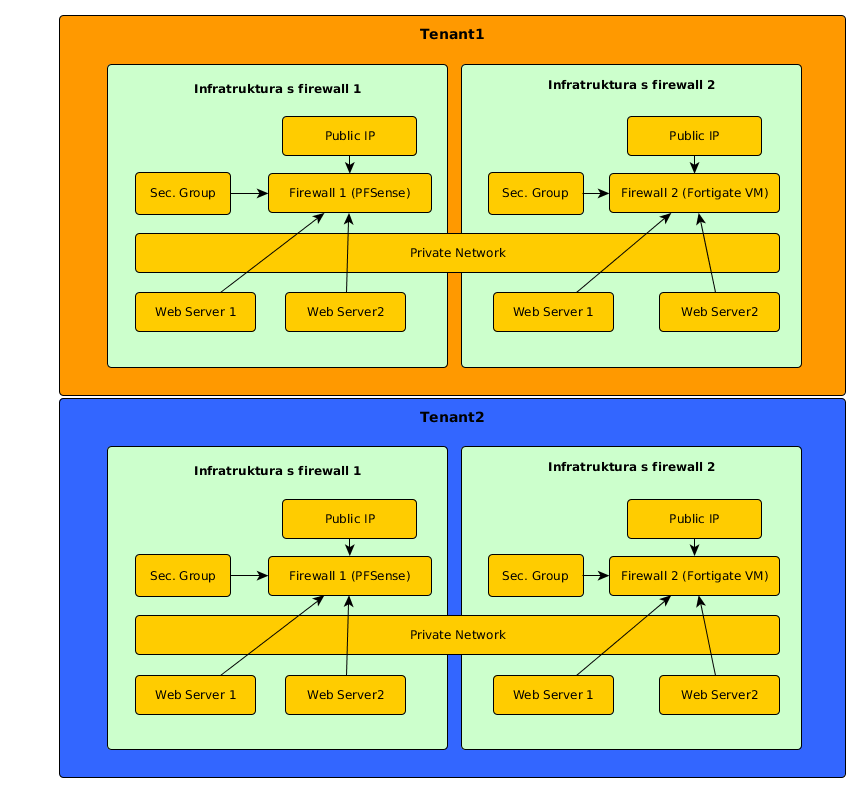
\includegraphics[scale=0.6]{images/firewall}
\par\end{centering}
\caption{Firewall as a Service\label{fig:firewall}}
\end{figure}

\section{Realizace VNF pro LbaaS}

\subsection{HAproxy - Neutron HAproxy agent}

OpenStack Neutron ve své implementaci obsahuje službu LBaaS. Je to jedna z jeho pokročilou služeb, která umožňuje použít jeden soubor API k ovládání load balanceru od poskytovatelů třetích stran. Jedinou podmínkou je, aby toto API implementovali. Toto velice zjednodušuje uživatelům OpenStacku ovládání load balancerů a odpadá díky tomu nutnost seznamování se s implementací a konfigurací těchto různých řešení, která mohou být velmi specifická a odlišná.

V této práci je ukázán příklad využítí implementace load balanceru v OpenContralu, který může být přes toto api ovládán. Tento příklad je však univerzální a může být použit s jakoukoli implementací load balanceru, at už virtuláního (sofwarového) či fyzického, pokud dokáže komunikovat s OpenStack Neutron LbaaS rozhraním. Dle dokumentace \cite{contrail_loadbalancer} je v OpenContrailu implementace load balanceru řešena pomocí HAProxy. HAProxy je zdarma dostupný open source software pro unix operační systémy \cite{HAProxy}. 

Load balancer se v Neutron LbaaS skládá ze 4 objektů.

\begin{itemize}
\item Pool - Označuje síťový rozsah pro webové servery.
\item Virtuální IP (VIP) - ip adresa, na kterou přichází komunikace
\item Member - Označuje konkrétní instanci, která je členem poolu.
\item Monitor - Monitoruje stav jednotlivých serverů a aplikací.
\end{itemize}

\begin{figure}[h]
\begin{centering}
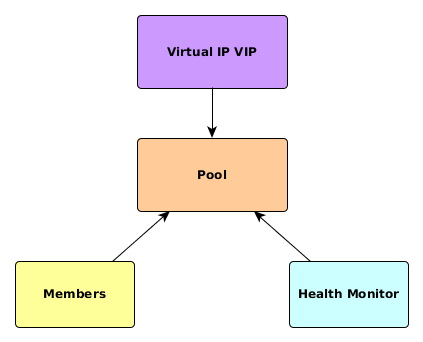
\includegraphics[scale=0.63]{images/NeutronLbaaS}
\par\end{centering}
\caption{Neutron LbaaS\label{fig:NeutronLbaaS}}
\end{figure}

Obrázek č. \ref{fig:NeutronLbaaS} zachycuje jednotlivé závislosti mezi těmito objekty. Tato implementace má tyto hlavní funkce:

\begin{itemize}
\item Poskytuje Load balancing komunikace od klientů do poolu serverů. Load balancer zprostředkovává spojení prostřednictvím své VIP.
\item Poskytuje load balancing pro HTTP, TCP a HTTPS komunikaci.
\item Poskytuje možnosti pro monitorování aplikací. Prostřednictvím HTTP, TCP či PING. Zde celý proces tak, že se load balancer pokusí v určeném časové intervalu navázat s daným serverem v pool spojení dle vybraného protokolu.
\item Umožňuje asociaci floating ip (veřejné adresy) k VIP, čímž umožňuje přístup k serverů z veřejné sítě.
\end{itemize}

Celý proces probíhá tak, že každý virtuální server, který je asociovaný s daným poolem z něj obdrží IP adresu. Když příjde na VIP nějaký dotaz na danou webovou aplikaci, tak je tento dotaz předán dál na jednu z těchto přiřazeným IP adres. Pokud nastane s aplikací či serverem nějaký problém, který zachytí monitor, tak load balancer ip adresu tohoto serveru přestane posílat komunikaci, dokud není vše zase v pořádku. Výběr serveru může probíhat pomocí jedné z následujících metod:

\begin{itemize}
\item Round robin - zde se komunikace distribuuje rovnoměrně, resp. dle vah zadaných u jednotlivých memberů v poolu.
\item Least connection - zde je vybran member s nejméně spojeními.
\item Source IP - u této metody je vybrán member na základě zdrojové ip adresy klienta.
\end{itemize}

V tomto případě si tedy není třeba starat o automatizaci konfigurace celého řešení. Je zde pouze nutné správně nadefinovat jednotlivé komponenty v heat templatu, abychom dosáhli požadovaného chování.

\subsubsection{LbaaS heat template}

Aby nemusel uživatel ručně vytvářet load balancer ručně, tak byl celý proces vytváření load balanceru zautomatizován pomocí heat templatu. Navržený heat template pro LbaaS v sobě obsahuje několik  prostředků, které se po jeho spuštění pokusí heat engine vytvořit. Celý template v sobě obsahuje i webové instance, které slouží pro testování. V produkci by však byly v odděleném templatu. Template je parametrizovaný a konktétní hodnoty pro jednotlivě zdroje (ip adresy, ip) jsou v tzv. enviroment file, který se zadává při spouštění daného templatu. Dále jsou popsány pouze hlavní části heat templatu.

\begin{itemize}
\item privatni síť - k této síti jsou připojeny obě webové instance, load balancer a router. Součástí je definice toho zdroje jsou je i subnet, který má dále paramentry týkající se DHCP ip adres.

\begin{lstlisting}[caption=Privátní síť a subnet]
private_net:
    type: OS::Neutron::Net
    properties:
      admin_state_up: True
      name: { get_param: private_net_name }
      shared: False
  private_subnet:
    type: OS::Neutron::Subnet
    properties:
      allocation_pools:
      - start: { get_param: private_net_pool_start }
        end: { get_param: private_net_pool_end }
      cidr: { get_param: private_net_cidr }
      enable_dhcp: True
      ip_version: 4
      name: { get_param: private_net_name }
      network_id: { get_resource: private_net }
\end{lstlisting}

\item 2 x web instance - jedná se o virtuální instance s operačním systémem Ubuntu 14.04. Po spuštění heat templatu se na tyto instance nainstaluje Apache server a vytvoří se index.html. Díky tomu je možné následně otestovat zda load balancer distubuje komunikaci mezi těmito dvěma servery.

\begin{lstlisting}[caption=Web server 1]
  instance_01:
    type: OS::Nova::Server
    properties:
      image: { get_param: instance_image }
      flavor: { get_param: instance_flavor }
      key_name: { get_param: key_name }
      name: test-web01
      networks:
      - network: { get_resource: private_net }
      security_groups:
      - default
      - { get_resource: http_security_group }
      user_data_format: RAW
      user_data: |
        #!/bin/bash -v
        apt-get install apache2 -yy
        echo "Instance 01" > /var/www/html/index.html
\end{lstlisting}


\item router - toto je Neutron router implementují SNAT. V tomto příkladě je využívaný webovými servery pro konektivitu k Internetu. Toto je nutné pro nainstalování programu Apache na webové servery.

\begin{lstlisting}[caption=Web server 1]
  router:
    type: OS::Neutron::Router
    properties:
      name: { get_param: router_name }
      external_gateway_info:
        network: { get_param: public_net_id }
\end{lstlisting}

\item public síť - toto je veřejná síť, ze které je získána VIP pro load balancer. Na tuto VIP bude dále asociována floating ip. 

\begin{lstlisting}[caption=Public síť a subnet]
  public_net:
    type: OS::Neutron::Net
    properties:
      admin_state_up: True
      name: { get_param: public_net_name }
      shared: False
  public_subnet:
    type: OS::Neutron::Subnet
    properties:
      allocation_pools:
      - start: { get_param: public_net_pool_start }
        end: { get_param: public_net_pool_end }
      cidr: { get_param: public_net_cidr }
      enable_dhcp: True
      ip_version: 4
      name: { get_param: public_net_name }
      network_id: { get_resource: public_net }
  lb_floating:
    type: OS::Neutron::FloatingIP
    properties:
      floating_network_id: {get_param: public_net_id}
      port_id: {get_attr: [lb_pool, vip, port_id]}
\end{lstlisting}

\item pool - jedná se o definování poolu pro load balancer. Na ukázce je vidět, že byla zvolena metoda Round Robin. Tato metoda byla zvolena kvůli co nejjednoduššímu testování tohoto templatu.

\begin{lstlisting}[caption=Load balancer pool]
  lb_pool:
    type: OS::Neutron::Pool
    properties:
      admin_state_up: True
      lb_method: ROUND_ROBIN
      name: { get_param: lb_name }
      protocol: HTTP
      monitors:
      - { get_resource: lb_ping_healt_monitor }
      subnet_id: { get_resource: private_subnet }
      vip:
        protocol_port: 80
        address: { get_param: public_net_ip }
        admin_state_up: True
        subnet: { get_resource: public_subnet }
\end{lstlisting}

\item members - po vytvoření instancí je nutné jejich přidání do poolu jako membery. Pokud webová aplikace na serverch využívá jiný port než port 80, je možné ho zde změnit.

\begin{lstlisting}[caption=Members]
  lb_pool_member_instance_01:
    type: OS::Neutron::PoolMember
    properties:
      address: { get_attr: [ instance_01 , first_address ] }
      admin_state_up: True
      pool_id: { get_resource: lb_pool }
      protocol_port: 80
\end{lstlisting}

\item health monitoring - zdroj pro monitoring. Dle zvolených parametrů je vidět, že každých 5 sekund bude poslán ping na servery a bude se čekat 5 sekund na odpověď. Pokud nepříjde, tak load balancer usoudí, že je daný server není v pořádku a přestane na něj přeposílat komunikaci.

\begin{lstlisting}[caption=Monitor]
  lb_ping_healt_monitor:
    type: OS::Neutron::HealthMonitor
    properties:
      admin_state_up: True
      delay: 5
      max_retries: 1
      timeout: 5
      type: PING
\end{lstlisting}
\end{itemize}

V celém heat templatu je ještě více zdrojů, které se vytváří. Ty zde však nebudou popsány. V případě zájmu lze nálest komletní heat template v příloze. 

\subsubsection{Testování LbaaS}\label{sub:interaction}

V reálné případě by si uživatel heat tempalte vybral z katalogu. Avšak v případě této práce bude heat template spouštěn pomocí příkazu v terminálu:

\begin{lstlisting}
heat stack-create -f heat/templates/lbaas_template.hot -e heat/env/lbaas_env.env lbaas
\end{lstlisting}

Tento příkaz vytvoří všechny již uvedené prostředky pro load balancing. Konkrétní load balancer má nakonfigurovanou virtual ip adresu (VIP) a k ní přiřazenou floating adresu, která je přístupná z externích sítí. Zároveň má tento load balancer přiřazený pool, ke kterému je přiřazena přiřazena privátní síť 10.10.10.0/24. Další zdrojem, který byl vytvořen je health monitor. Díky němu má load balancer přehled o aktuálním stavu webových instancí. Pokud by náhodou některá z nich přestala odpovídat, v tomto případě na ping, tak by load balancer na tuto instanci přestal zasílat traffic.

Na obrázku č. \ref{fig:lbaas_topologie} je zobrazek screenshot vytvořené topologie v OpenStack dashboardu. Jsou zde vidět vytvořené servery a sítě. Není zde zobrazen load balancer, protože tato vizualizace tento prvek nezobrazuje. Lze ho nalézt v jiné části dashboardu, ale pro názornost bude rovnou otestováno jeho správné chování.

\begin{figure}[h]
\begin{centering}
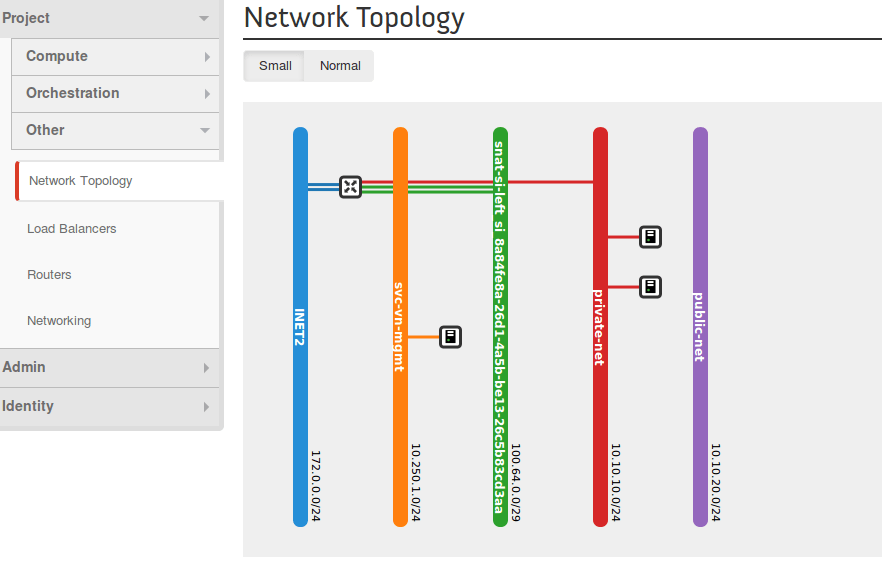
\includegraphics[scale=0.45]{images/lbaas_topologie}
\par\end{centering}
\caption{Vytvořená síťová topologie\label{fig:lbaas_topologie}}
\end{figure}

Otestování správného chování virtuálního load balanceru, lze provést opakovaným dotazem na právě vytvořené webové servery. Tím je bude zároveň otestována jejich správná konfigurace. Pokud by totiž nevrátili správnou odpoveď je možné, že chyba může být i zde. 

Dotaz na webové servery byl proveden pomocí příkazu curl, kterému byla dána jako parametr public adresa load balanceru. Celý výstup toho testování znázorňuje obrázek č. \ref{fig:lbaas_testing}. Po několika takovýchto dotazech na webové servery je vidět, že odpověď příchází střídavě od obou webových serverů. Probíhá mezi nimi tedy load balancing metodou round robin tak, jak bylo požadováno.

\begin{figure}[h]
\begin{centering}
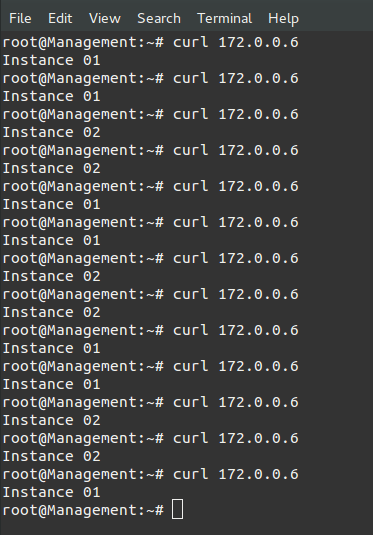
\includegraphics[scale=0.3]{images/lbaas_testing}
\par\end{centering}
\caption{Test konektivity a load balancingu\label{fig:lbaas_testing}}
\end{figure}


\subsection{AVI networks}




\section{Realizace VNF pro FwaaS}

\subsection{Servisní instance v OpenContrailu}

V OpenContrailu je sice možnost využívat implementaci routeru s SNAT, která umožnuje instancím v privátních sítích konektivitu s externí sítí. Pokud však uživatel potřebuje využít pokročilejší funkce firewallu, tak je možné vytvořit servisní instanci, která bude sloužit jako VNF. V té může být použit libovolný požadovaný image firewallu uživatele.

Servisní instance v OpenContrailu je jednoduše virtuální stroj, který poskytuje danou VNF. Úplně nejjednodušším příkladem může být virtuální stroj s operačním systémem GNU/Linux, který může sloužit jako router mezi dvěma sítěmi. Pro vytvoření takového virtuálního stroje jsou nutné 3 základní elementy. 

\begin{itemize}
  \item Service Template
  \item Service Instance
  \item Service Policy
\end{itemize}

Servisní Template obsahuje obecný předpis pro danou VNF v OpenContrailu. Pro správné fungování je nutné zadat nastavit správné parametry patří:

\begin{itemize}
\item Název - Název je označení daného Servisního Templatu. Pomocí něho lze následně identifikovat daný template a spustit dle jeho parametrů Servisní instanci. 
\item Image - Je image, který má být použit pro vytvoření dané servisní instance. V našem případě se bude jednat o image, který obsahuje požadované síťové funkce. Tento image musí před tím než může být použit  nahrán do OpenStacku Glance.
\item Service Type - V OpenContrailu, prozatím existují dva typy. Jsou to Trafic Analyzer a Firewall.
\item Service Mode - Zde se určuje v jakém modu daný template bude nastaven. Jsou zde 3 možnosti. , .

  \begin{itemize}
  \item Transparent - v tomto případě se jedná o neroutovaný firewall, neboli L2 firewall.
  \item In-Network - poskytuje výchozí bránu a průchozí traffic je routovaný. Tento mode může být využit pro NAT, HTTP proxy, atd.
  \item In-Network-NAT - zde je situace podobná jako u In-Network, ale navracející traffic nemusí být routovaný zpět do zdrojové sítě.
  \end{itemize}

\item Typy síťových portů - Zde se určuje kolik portů bude daná instance, vytvořená pomocí tohoto templatu mít a jaká bude jejich role. Jsou zde možnosti Left, Right a Management. 
\end{itemize}

Po úspěšném vytvoření Servisního templatu je možné z něj vytvořit libovolný počet Servis Instancí.  Ty běží jako klasické instance v OpenStacku. Jak tedy vyplývá z výše uvedených informací, tak existují dva druhy servisních instancí v OpenContrailu. 

První z nich je Analyzer. Ten slouží k analýze a zachytávání síťového trafficu. Image pro tento typ servisní instance obvykle obsahuje protokolový analyzér a paketový sniffer, jako je například oblíbený program Wireshark. Tato instance dostává traffic, který je posílán mezi dvěma sítěmi. Tento traffic vybírá OpenContrail podle nastaveného pravidla pro dané sítě. Podle těchto pravidel je vybrána jen část trafficu, která je následně dána k dispozici servisní instanci. Samotná servisní instance nijak nemanipuluje s trafficem a ani do něj žádný negeneruje. Jednoduše lze říci, že má nastavený síťový port v promiskuitním modu a pouze pozoruje traffic. Poté jen hlásí zachycené události uživateli čí jiným entitám v síti. Obrázek č. \ref{fig:service_instance_anal} znázorňuje tento typ servisní instance.

\begin{figure}[h]
\begin{centering}
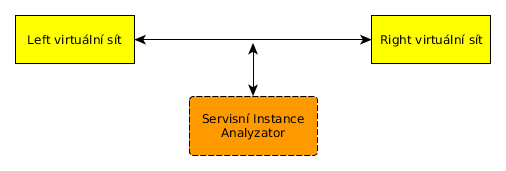
\includegraphics[scale=0.63]{images/service_instance_anal}
\par\end{centering}
\caption{Schéma zapojení servisní instance Analyzer\label{fig:service_instance_anal}}
\end{figure}

Druhým typen servisní instance je firewall. V tomto případě již servisní instance manipuluje s trafficem. Hlavní bodem při vytváření servisní instance jako firewall je přiřadit správné virtuální sítě k správným virtuálním síťovým portům. Servisní instance má obvykle dva síťové porty - left a right. Ty slouží pro propojení sítí do kterých jsou zapojeny. V některých případech je možné servisní instanci přidat třetí síťový port, který slouží pro out-of-band management. Přestože některá řešení pro servisní instance sloužící jako firewall mohou mít již své požadované chování definované hned při jejich startu, tak tento port může být velice užitečný při konfiguraci dané servisní instance. A to ať už se jedná o konfiguraci manuální či pomocí nějaké vyšší management entity.

\begin{figure}[h]
\begin{centering}
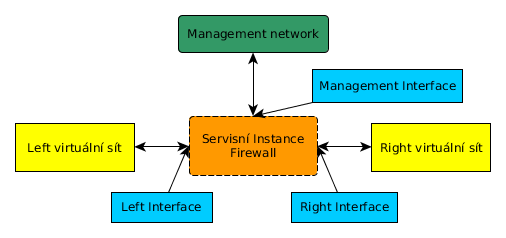
\includegraphics[scale=0.63]{images/service_instance}
\par\end{centering}
\caption{Schéma zapojení servisní instance\label{fig:service_instance}}
\end{figure}


Service policy dovoluje síťový traffic mezi virtuálními sítěmi a říká systému, aby ho posílal skrze servisní instanci.


\subsection{Heat template pro FwaaS}

Pro FwaaS je narhnut heat template, který obsahuje:

\begin{itemize}

\item privátní síť


\begin{lstlisting}[caption=Privátní síť]
  private_net_1:
    type: OS::Neutron::Net
    properties:
      name: { get_param: private_net_1_name } 

  private_subnet_1:
    type: OS::Neutron::Subnet
    depends_on: private_net_1
    properties:
      network_id: { get_resource: private_net_1 }
      cidr: { get_param: private_net_1_cidr }
      gateway_ip: { get_param: private_net_1_gateway }
      allocation_pools:
        - start: { get_param: private_net_1_pool_start }
          end: { get_param: private_net_1_pool_end }
\end{lstlisting}


\item firewall template

\begin{lstlisting}[caption=Firewall servisní instance]
service_template:
    type: OS::Contrail::ServiceTemplate
    properties:
      name: { get_param: template_name }
      service_mode: { get_param: template_mode }
      service_type: { get_param: template_type }
      image_name: { get_param: template_image }
      service_scaling: { get_param: scaling }
      availability_zone_enable: { get_param: availability_zone }
      ordered_interfaces: { get_param: ordered_interfaces }
      flavor: { get_param: template_flavor }
      service_interface_type_list: { "Fn::Split" : [ ",", Ref: service_interface_type_list ] }
      shared_ip_list: { "Fn::Split" : [ ",", Ref: shared_ip_list ] }
      static_routes_list: { "Fn::Split" : [ ",", Ref: static_routes_list ] }

\end{lstlisting}

\item firewall instance
\begin{lstlisting}[caption=Privátní síť]
 service_instance:
    type: OS::Contrail::ServiceInstance
    depends_on: [private_subnet_1]
    properties:
      name: { get_param: private_instance_name }
      service_template: { get_resource:  service_template}
      availability_zone: { get_param: private_availability_zone}
      scale_out: 
          max_instances: { get_param: max_instances }
      interface_list: [
          {
              virtual_network: "auto"
          },
          {
              virtual_network: {get_param: public_net}
          },
          {
              virtual_network: {get_resource: private_net_1}
          }
      ]
\end{lstlisting}


\item virtuální instance
\begin{lstlisting}[caption=Virtuální instance pro testování]

 test_instance_01:
    type: OS::Nova::Server
    properties:
      image: { get_param: instance_image }
      flavor: { get_param: instance_flavor }
      key_name: { get_param: key_name }
      name: test-web01
      networks:
      - network: { get_resource: private_net_1 }
      security_groups:
      - default
      user_data_format: RAW
      user_data: |
        #!/bin/bash -v
        apt-get install apache2 -yy
        echo "Instance 01" > /var/www/html/index.html

\end{lstlisting}

\item contrail policy

\begin{lstlisting}[caption=Contrail network policy]

  private_policy:
    type: OS::Contrail::NetworkPolicy
    depends_on: [ private_net_1, service_instance ]
    properties:
      name: { get_param: policy_name }
      entries:
        policy_rule: [
              { 
                "direction": { get_param: direction }, 
                "protocol": "any", 
                "src_ports": [{"start_port": {get_param: start_src_ports}, "end_port": {get_param: end_src_ports}}],
                "dst_ports": [{"start_port": {get_param: start_dst_ports}, "end_port": {get_param: end_dst_ports}}],
                "dst_addresses": [{ "virtual_network": {get_param: public_net}}], 
                "action_list": {"apply_service": [{get_resource: service_instance}]}, 
                "src_addresses": [{ "virtual_network": {get_resource: private_net_1}}] 
              }, 
        ]

\end{lstlisting}
\end{itemize}

\subsection{PfSense}\label{sub:interaction}

Pro vytvoření heat stacku s PFSense z templatu lze použít příkaz:

\verb!heat stack-create -f heat/templates/fwaas_mnmg_template.hot -e heat/env/fwaas_pfsense_env.env pfsense!

a pro vytvoření heat stacku s Fortigate VM jde vytvořit pomocí příkazu:

\verb!heat stack-create -f heat/templates/fwaas_mnmg_template.hot -e heat/env/fwaas_fortios_contrail.env fortios!


\begin{figure}[h]
\begin{centering}
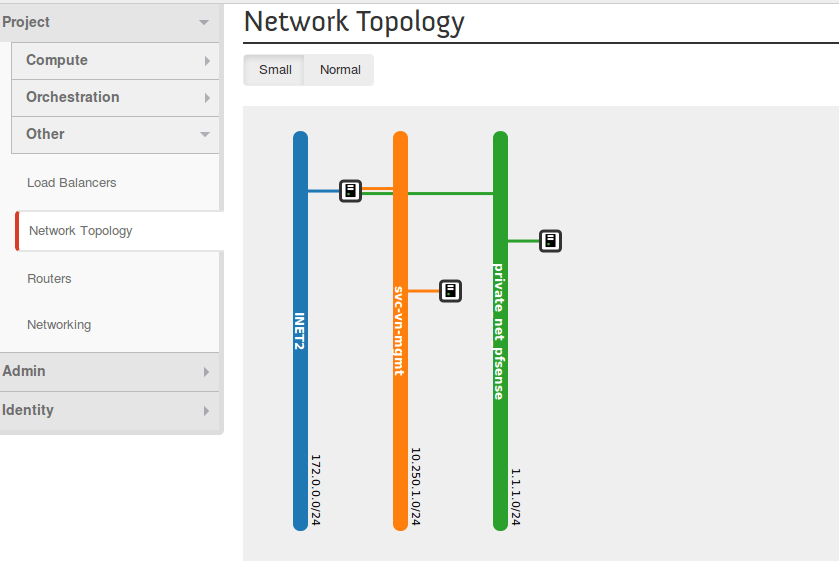
\includegraphics[scale=0.45]{images/fwaas_topologie}
\par\end{centering}
\caption{Síťová topologie\label{fig:fwaas_topologie}}
\end{figure}


By default, pfsense firewall is configured to NAT after the heat stack is started. As a result, there is no need to make any configuration for this function. Pfsense image was preconfigured with DHCP services on every interface and there is outbound policy for NAT.

After we start the heat with pfsense there is already functional service chaining. Testing instance has default gateway to contrail and contrail redirects it to pfsense.

\begin{figure}[h]
\begin{centering}
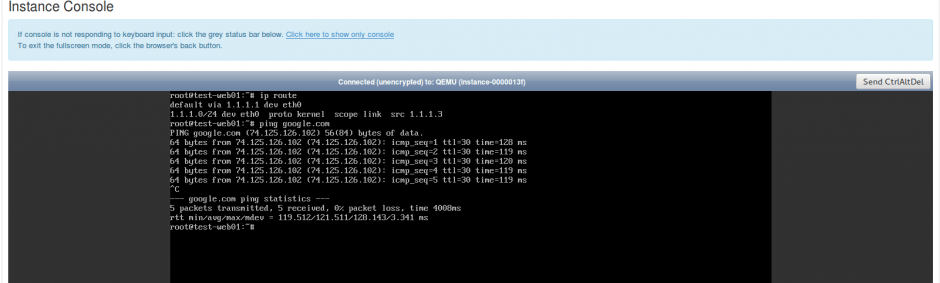
\includegraphics[scale=0.45]{images/pfsense_ping}
\par\end{centering}
\caption{Test konektivity PFSense\label{fig:pfsense_ping}}
\end{figure}

\begin{figure}[h]
\begin{centering}
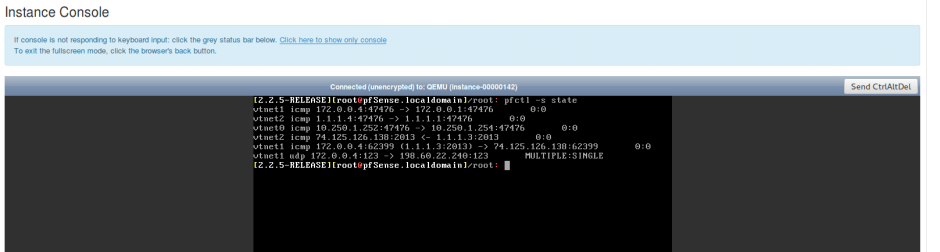
\includegraphics[scale=0.45]{images/pfsense_nat}
\par\end{centering}
\caption{Ukázka NAT session\label{fig:pfsense_nat}}

//Bash script nefunguje
//Predpripraveny image

\subsection{Fortigate}

//Python API = Script
// => Salt module 
\end{figure}

\begin{figure}[h]
\begin{centering}
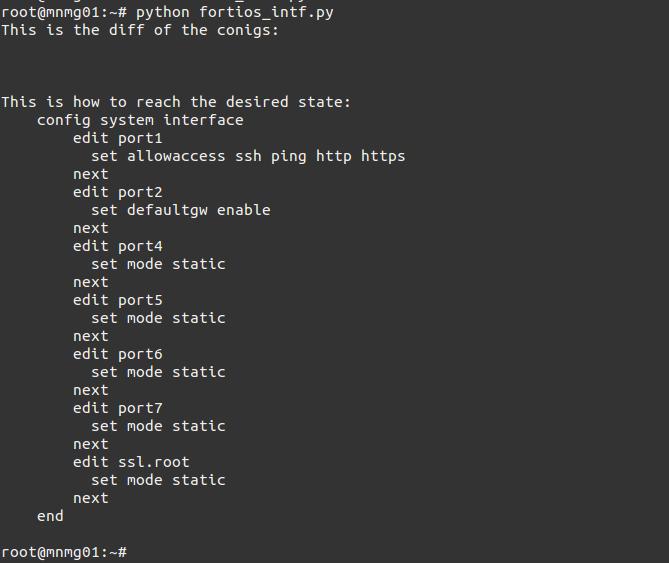
\includegraphics[scale=0.45]{images/fortigate_int}
\par\end{centering}
\caption{Fortigate VM intergace konfigurace\label{fig:fortigate_int}}
\end{figure}

\begin{figure}[h]
\begin{centering}
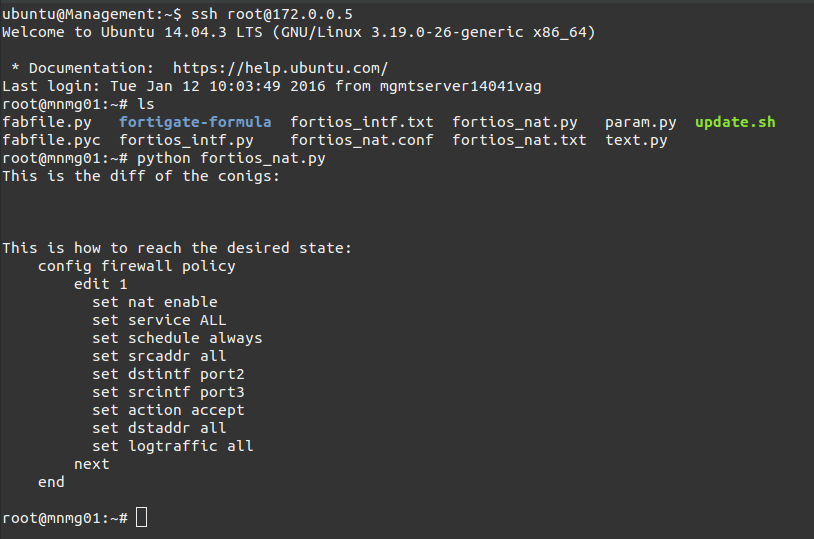
\includegraphics[scale=0.45]{images/fortigate_nat}
\par\end{centering}
\caption{Fortigate VM NAT konfigurace\label{fig:fortigate_nat}}
\end{figure}

\begin{figure}[h]
\begin{centering}
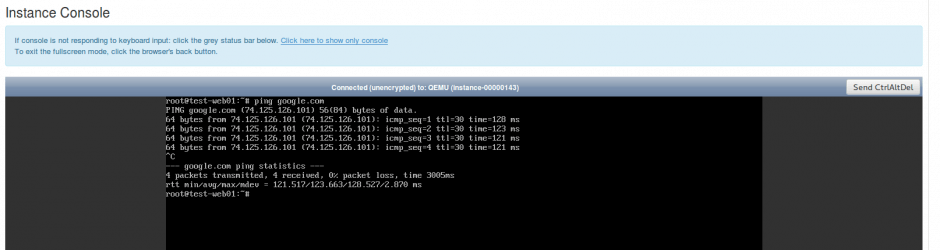
\includegraphics[scale=0.45]{images/fortigate_ping}
\par\end{centering}
\caption{Test konektivity\label{fig:fortigate_ping}}
\end{figure}

